%Ukazka zaverecne zpravy
%Posledni zmena 02/2018, Martin Cadik

\documentclass[11pt,a4paper,oneside]{article}
\usepackage[utf8]{inputenc}
\usepackage{a4wide}
\usepackage{url}
\usepackage[breaklinks=true,hidelinks]{hyperref}
%\usepackage[chapter]{algorithm}
%\floatname{algorithm}{Alg.} 
\usepackage{ifpdf}
\ifpdf
\usepackage[pdftex]{graphicx}
\DeclareGraphicsExtensions{.pdf,.png,.gif,.jpg}
\else
\usepackage[final]{graphicx}
\DeclareGraphicsExtensions{.eps,.png,.gif,.jpg}
\fi 
\graphicspath{{fig/}}
\usepackage[export]{adjustbox}


% TODO Jak moc mám přepisovat ten článek.
% TODO jak moc chce popisovat tu implementaci
% TODO uživatelská studie - to mám ukázat metodu lidem a říct mi, která se jim
% líbí víc?

\begin{document}

\thispagestyle{empty}
\begin{center}
\vspace*{60mm}
{Semestrální projekt předmětu Výpočetní fotogragie -- závěrečná zpráva }\\
\smallskip
{\Large\bf Tone Mapping: implementace algoritmu Khan20}\\
\smallskip
{\it Milan Tichavský, \url{xticha09@fit.vut.cz}}\\
\vfill
{\bf Vedoucí práce:} {\it doc. Ing. Martin Čadík, Ph.D., \url{cadik@fit.vut.cz}} 
\hfill {Květen 2025}


\end{center}
\newpage


\section{Úvod}

Zařízení běžně používaná k zobrazování digitálního obsahu, jako jsou monitory,
televizory a tiskárny, nejsou schopna zobrazit celý dynamický rozsah světla
přítomného v reálném světě. Z tohoto důvodu existují metody pro převod obrazu s
vysokým dynamickým rozsahem (HDR) na standardní dynamický rozsah (SDR), aby ho bylo
možné správně vizualizovat na dostupných zařízeních. Tento proces se nazývá
\emph{tone mapping}.

Cílem této práce je implementace a analýza jednoho z moderních \emph{tone
mapping} algoritmů, konkrétně metody Khan20~\cite{Khan2020}, jako pluginu do Tone Mapping
Studia (TMS)~\cite{TMS2025}.

\section{Teoretické základy}

Pro pochopení \emph{tone mappingu} je nutné zmínit základní vlastnosti lidského
vidění. Lidské oko dokáže adaptivně vnímat velký rozsah jasových hodnot díky
nelineárnímu vnímání jasu a kontrastu. Toto umožnuje transformovat každou část
spektra s jinou přesností a tím lépe využít výstupní rozsah hodnot za zachování
co nejvíce detailů.

\section{Popis algoritmu Khan20}

Algoritmus Khan20 je globální \emph{tone mapping} operátor (TMO), to znamená že pro
transformaci je využita monotónní neklesající mapovací funkce. 
Algoritmus je založený na transformaci obrazu pomocí funkce \textit{Perceptual
Quantizer (PQ)} a histogramu jasu. Schéma algoritmu je vidět na obrázku
\ref{fig:schema}.

\begin{figure}[htb]
  \begin{center}
    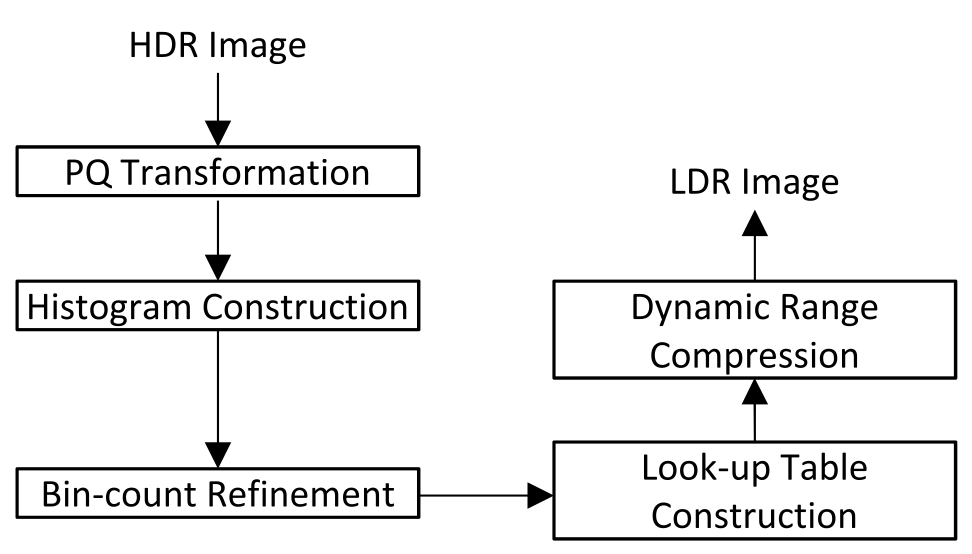
\includegraphics[width=0.8\linewidth]{fig/schema.png}
      \caption{Schéma algoritmu převzato z článku Khan20~\cite{Khan2020}.} 
    \label{fig:schema}
  \end{center}
\end{figure}

Funkce PQ se snaží simulovat vnímaní lidského oka a transformuje vstupní jas v
rozsahu $[0, 10000]$ cd/m$^2$ na normalizovaný rozsah $[0,1]$, přičemž nižší
jasové hodnoty mají k dispozici větší relativní rozlišení.

Výstup po transformaci je ukázán v tabulce \ref{tab:method-pq}. Je vidět, že z
takto transformovaného obrázku lze jasně vidět celou scénu, která ale působí
vybledle a má relativně nízký kontrast.

\begin{table}[htb]
    \centering
    \caption{Obrázky po transformaci funkcí \textit{Perceptual Quantizer}.}
    \label{tab:method-pq}
    \begin{tabular}{lll}
        \includegraphics[width=.33\linewidth,valign=m]{churchKhanPQ.png} &
        \includegraphics[width=.33\linewidth,valign=m]{buildingKhanPQ.png} &
        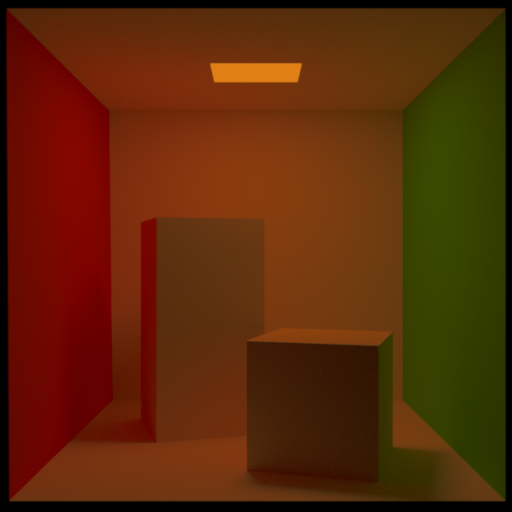
\includegraphics[width=.33\linewidth,valign=m]{cornell_boxKhanPQ.png} \\
    \end{tabular}
\end{table}

Z toho důvodu je v druhém kroku algoritmu zkonstruován histogram jasů, ze
kterého je vytvořena vyhledávací tabulka. Podle této tabulky se poté provádí
mapování hodnoty každého vstupního pixelu na hodnotu výstupní. Počet řádků je
dán parametrem $N$ (v příkazové řádce TMS lze zadat přepínačem \texttt{-Bins}),
přičemž implicitní hodnota je 256.

Už dříve bylo zjištěno, že použití klasického histogramu je problematické,
protože se může stát, že malým oblastem přiřadí moc malý výsledný rozsah.
Například pokud máme čistě modrou oblohu zabírající velkou část snímku,
nechceme, aby zabírala půlku výsledného rozsahu jasu, protože jas všech pixelů
bude velmi podobný. Proto je nutné
omezit počet pixelů v každém intervalu (\textit{bin}) pomocí parametru $ k $, kde
$k/N*pixel\_count$ je maximální počet pixelů pro každý interval. S pixelama které
se do daného počtu nevlezou, se nic neděje, akorát pro další výpočty je počet
pixelů v daném intervalu podhonocen. V TMS lze parametr $ k $ nastavit přepínačem
\texttt{-Truncation} s implicitní hodnotou 5.

\subsection{Ukládání výsledného obrázku}

Zatímco na vstupu algoritmu se předpokládá RGB obrázek, výstup algoritmu jsou
transformované úrovně jasu pro každý pixel. V článku bohužel není uvedeno, jak
přesně tento výstup převést do výsledného souboru. Proto jsem zvolil to co
považuji za standardní postup, tedy obrázek na vstupu jsem převedl do Yxy barevného
prostoru, nahradil jasovou složku nově vypočtenými hodnotami a výsledek uložil
jako výsledek algoritmu. Pro transformaci do Yxy jsem využil vestavěných metod
Tone Mapping Studia.

\section{Implementace a výpočetní složitost}

Výpočetní složitost implementace je nízká, program projde celkem 4x
přes všechny pixely obrázku a v každém kroku provede relativně jednoduché výpočty. 
Počet průchodů by šel snížit, nicméně chtěl jsem nechat kód co nejpřehlednější,
takže se každá funkce mapuje na jednu fázi algoritmu.

Z hlediska optimalizací je nejzajímavější implementace vyhledávání v lookup
tabulce, pro které jsem použil \texttt{std::upper\_bound} nad vektorem.
Tato funkce sice pracuje s iterátory, což dělá zápis trochu komplikovanější,
ale umožňuje nám dělat vyhledávání v LUT s \emph{log N} složistostí,
což je za mě klíčové, vzhledem k tomu, že se tato operace provádí pro každý
pixel obrázku.

\section{Výsledky}

% Nejdůležitější část -- diskuse výsledků, 
% načtené/vypozorované klady a zápory, operační složitost, ...
% Ukázkové obrázky.


\begin{table}[htb]
    \centering
    \caption{Srovnání různých metod; ve sloupcích zleva doprava jsou Khan20,
    Drago03 a Ward94. Všechny spouštěny s výchozíma hodnotama parametrů v Tone Mapping
    Studiu.}
    \label{tab:method-comp}
    \begin{tabular}{lll}
        \includegraphics[width=.33\linewidth,valign=m]{churchKhan20.png} &
        \includegraphics[width=.33\linewidth,valign=m]{churchDrago03.png} &
        \includegraphics[width=.33\linewidth,valign=m]{churchWard94.png} \\
    \includegraphics[width=.33\linewidth,valign=m]{buildingKhan20.png} &
        \includegraphics[width=.33\linewidth,valign=m]{buildingDrago03.png} &
        \includegraphics[width=.33\linewidth,valign=m]{buildingWard94.png}\\
    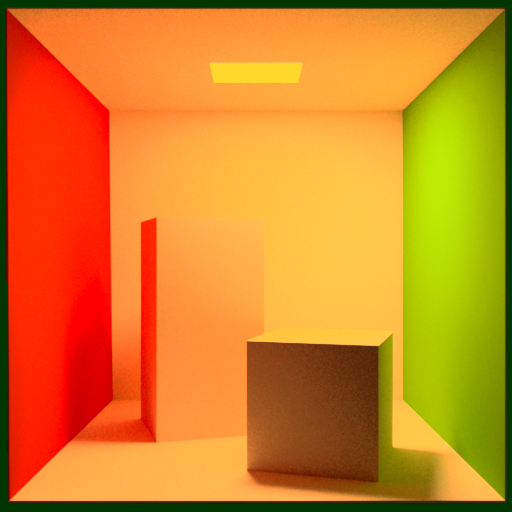
\includegraphics[width=.33\linewidth,valign=m]{cornell_boxKhan20.png} &
        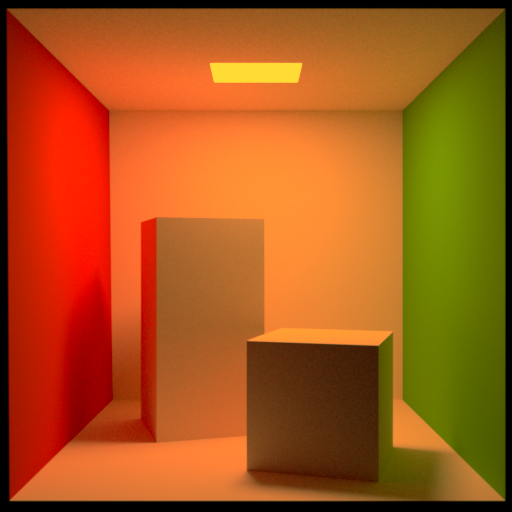
\includegraphics[width=.33\linewidth,valign=m]{cornell_boxDrago03.png} &
        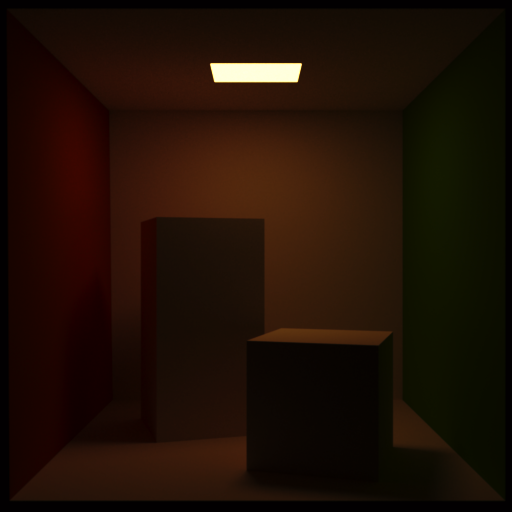
\includegraphics[width=.33\linewidth,valign=m]{cornell_boxWard94.png}\\
    \end{tabular}
\end{table}


V tabulce \ref{tab:method-comp} je vidět porovnání různých metod. Zvolil jsem ty
metody, které ve výchozím nastavení byly schopny rozumně zobrazit všechny tři
obrázky.

Jak je vidět, na všech obrázcích jsou scény krásně viditelné. V žádném případě
nebylo nutné jakkoliv přenastavovat výchozí parametry, což považuji za jednu z
velkých výhod tohoto algoritmu oproti ostatním, které jsem zkoušel a musel
parametry často upravovat.

Z metod v tabulce 2 se mi subjektivně nejvíc líbí Drago03, protože tmavé části
jsou opravdu tmavé a barvy mi taky přijdou přirozenější. Například strop kostela je 
pro výstup Khan20 v hodně oranžovém odstínu. Na druhou stranu se světlejší barvy hodí pro chodbu
druhého testovacího obrázku, kde jsou díky tomu lépe vidět detaily. Líbí se mi i
záře kolem okna kostela, která je jednoznačně nejsvítivějším místem celé scény.

\section{Závěr}

V rámci projektu jsem implementoval plugin Khan20 do Tone Mapping studia a
porovnal jeho algoritmus s ostatními metodami. Výsledky ukazují, že algoritmus
funguje velmi dobře pro různé scény s výchozími parametry. Výstupní snímky jsou
o něco světlejší a možná méně saturované, než bych si přál z uměleckého
hlediska. Na druhou stranu metoda vyniká v zobrazování detailů, a to i v tmavých
oblastech. Díky tomu jsou detaily lépe viditelné i při odlescích na monitoru
nebo v přítomnosti silného externího osvětlení, což může být výhoda v různých
aplikacích.

\bibliographystyle{acm}
\bibliography{report}

\end{document}
